\section{Luminotécnica}


\begin{frame}{Introdução}
	\begin{block}{Conceitos iniciais}
		\begin{itemize}
			\item À época do surgimento do homem primitivo, a raça humana vivia entre o \textbf{medo da noite} e a sua \textbf{sobrevivência}.
		\end{itemize}
	\end{block}

	\centering
	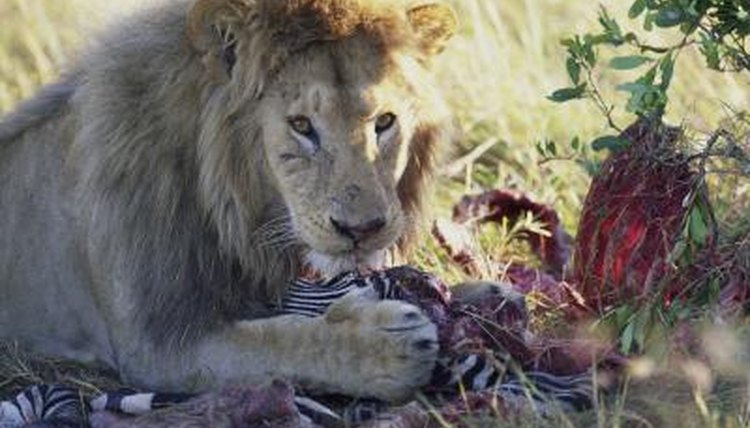
\includegraphics[width=0.85\linewidth]{Figuras/Ch07/fig1.2}

\end{frame}


\begin{frame}{Introdução}
	\begin{block}{Conceitos iniciais}
		\begin{itemize}
			\item Depois de dominar o fogo, além de ganhar um poderoso aliado contra seus inimigos naturais - as \textbf{feras} e o \textbf{frio} - nossos ancestrais passaram a usar parte da noite, agora \textbf{iluminada} pelas fogueiras e tochas, para algumas atividades de \textbf{artesanato} e principalmente para o \textbf{convívio}.
		\end{itemize}
	\end{block}

	\centering
	
\includegraphics[width=0.6\linewidth]{Figuras/Ch07/fig1.1}

\end{frame}


\begin{frame}{Introdução}
	\begin{block}{Conceitos iniciais}
		\begin{itemize}
			\item Podemos dizer que todo o \textbf{desenvolvimento} da espécie humana começou com a \textbf{conquista do fogo e da luz}.
			\item Há milhares de anos estamos \textbf{desenvolvendo métodos} para \textbf{melhor aproveitar a luz}, sempre visando o \textbf{conforto visual} e a \textbf{sustentabilidade}.
		\end{itemize}
	\end{block}

	\bigskip
	\centering
	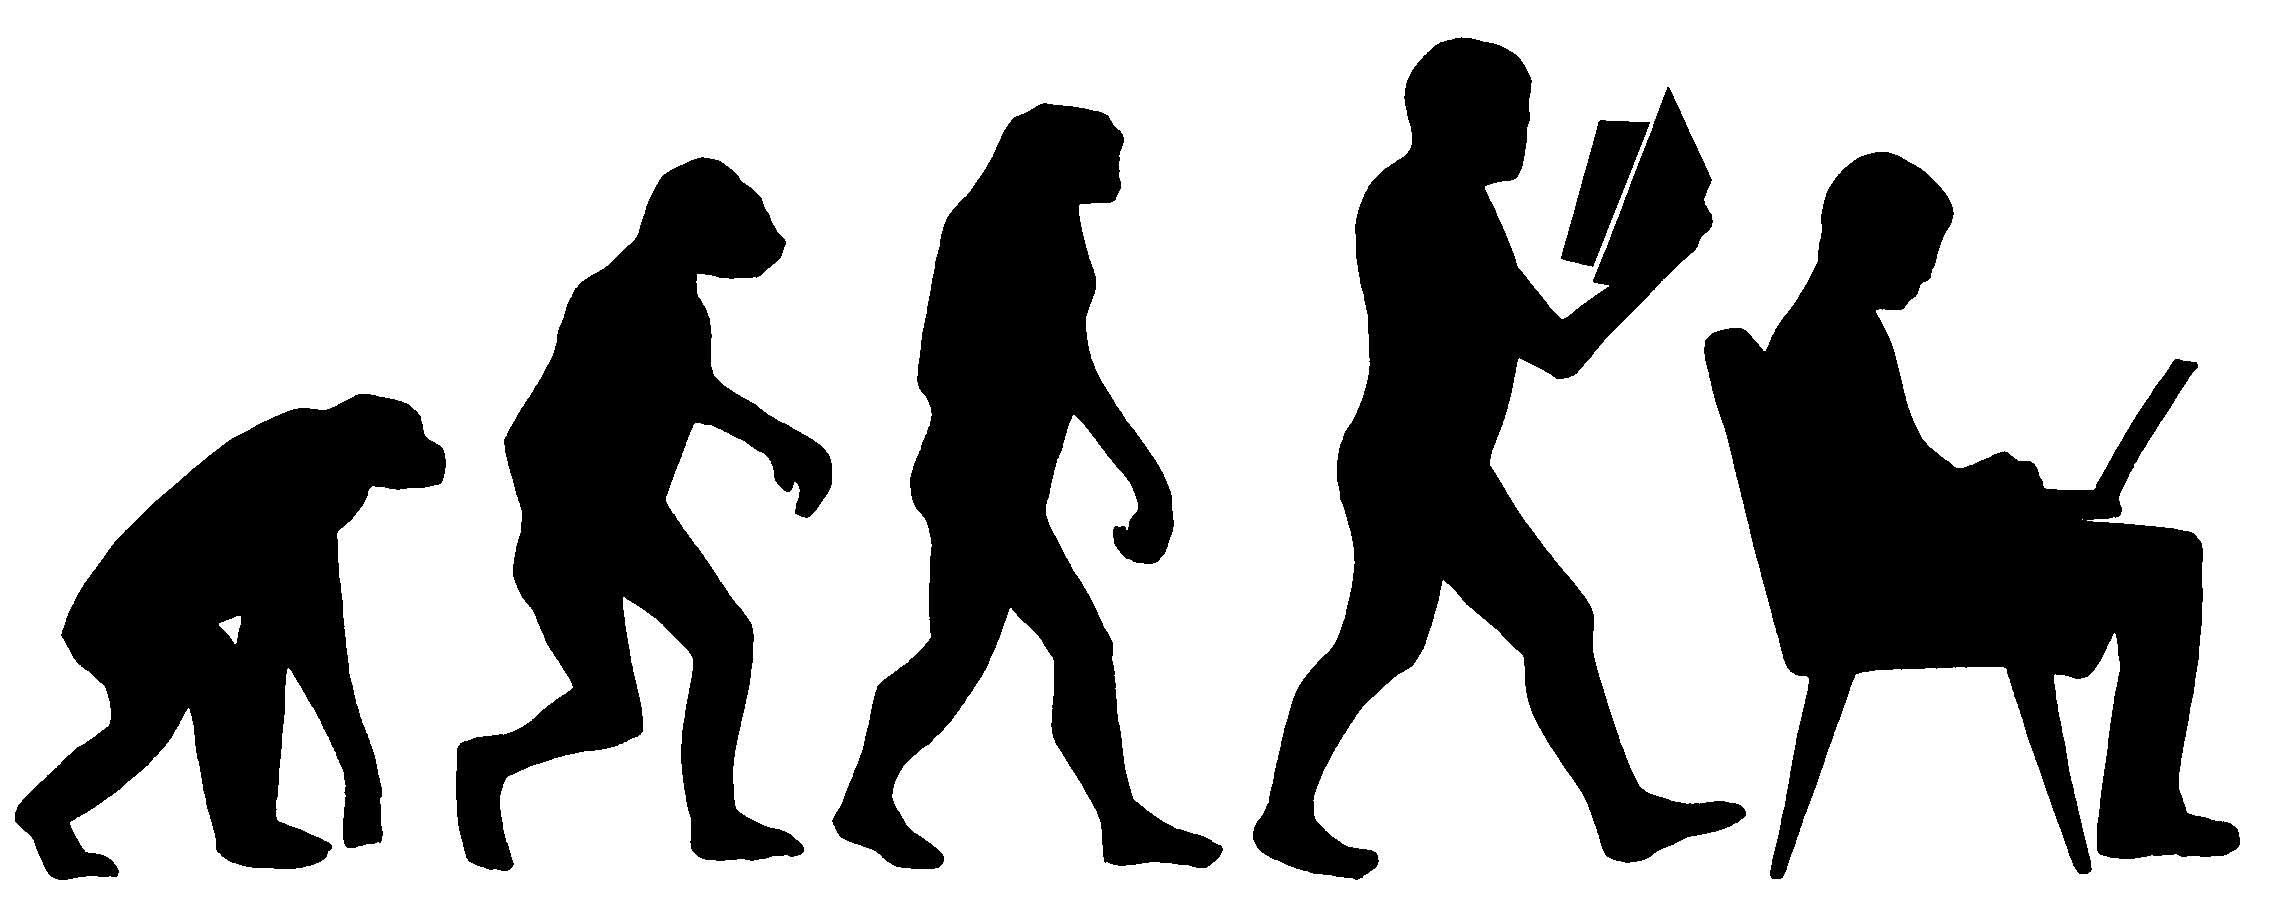
\includegraphics[width=0.8\linewidth]{Figuras/Ch07/fig1.3}

\end{frame}


\begin{frame}{Introdução}
	\begin{block}{Conceitos iniciais}
		\begin{itemize}
			\item Outro aspecto \textbf{fundamental} é a utilização da luz para \textbf{destacar} e \textbf{embelezar as construções}.
			\item A arquitetura religiosa usou os efeitos gerados pela luz solar para criar \textbf{atmosferas místicas} e \textbf{mágicas} dentro de seus templos.
			\item Nesse caso a função da luz \textbf{não era apenas iluminar}, mas sim \textbf{criar emoções}, tanto de \textbf{adoração e reverência} nas \textbf{igrejas}, quanto impressões de \textbf{admiração estética} nos \textbf{palácios}.
		\end{itemize}
	\end{block}
\end{frame}


\begin{frame}{Introdução}
	\centering
	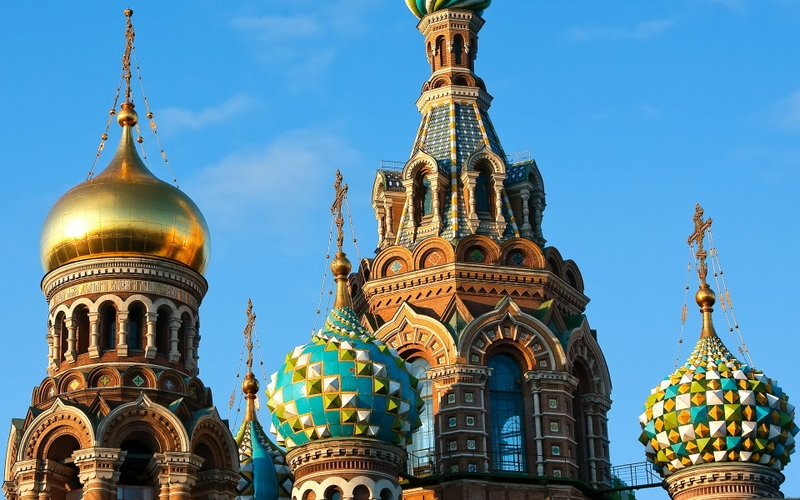
\includegraphics[height=0.9\textheight]{Figuras/Ch07/fig1.4}
\end{frame}


\begin{frame}{Introdução}
	\centering
	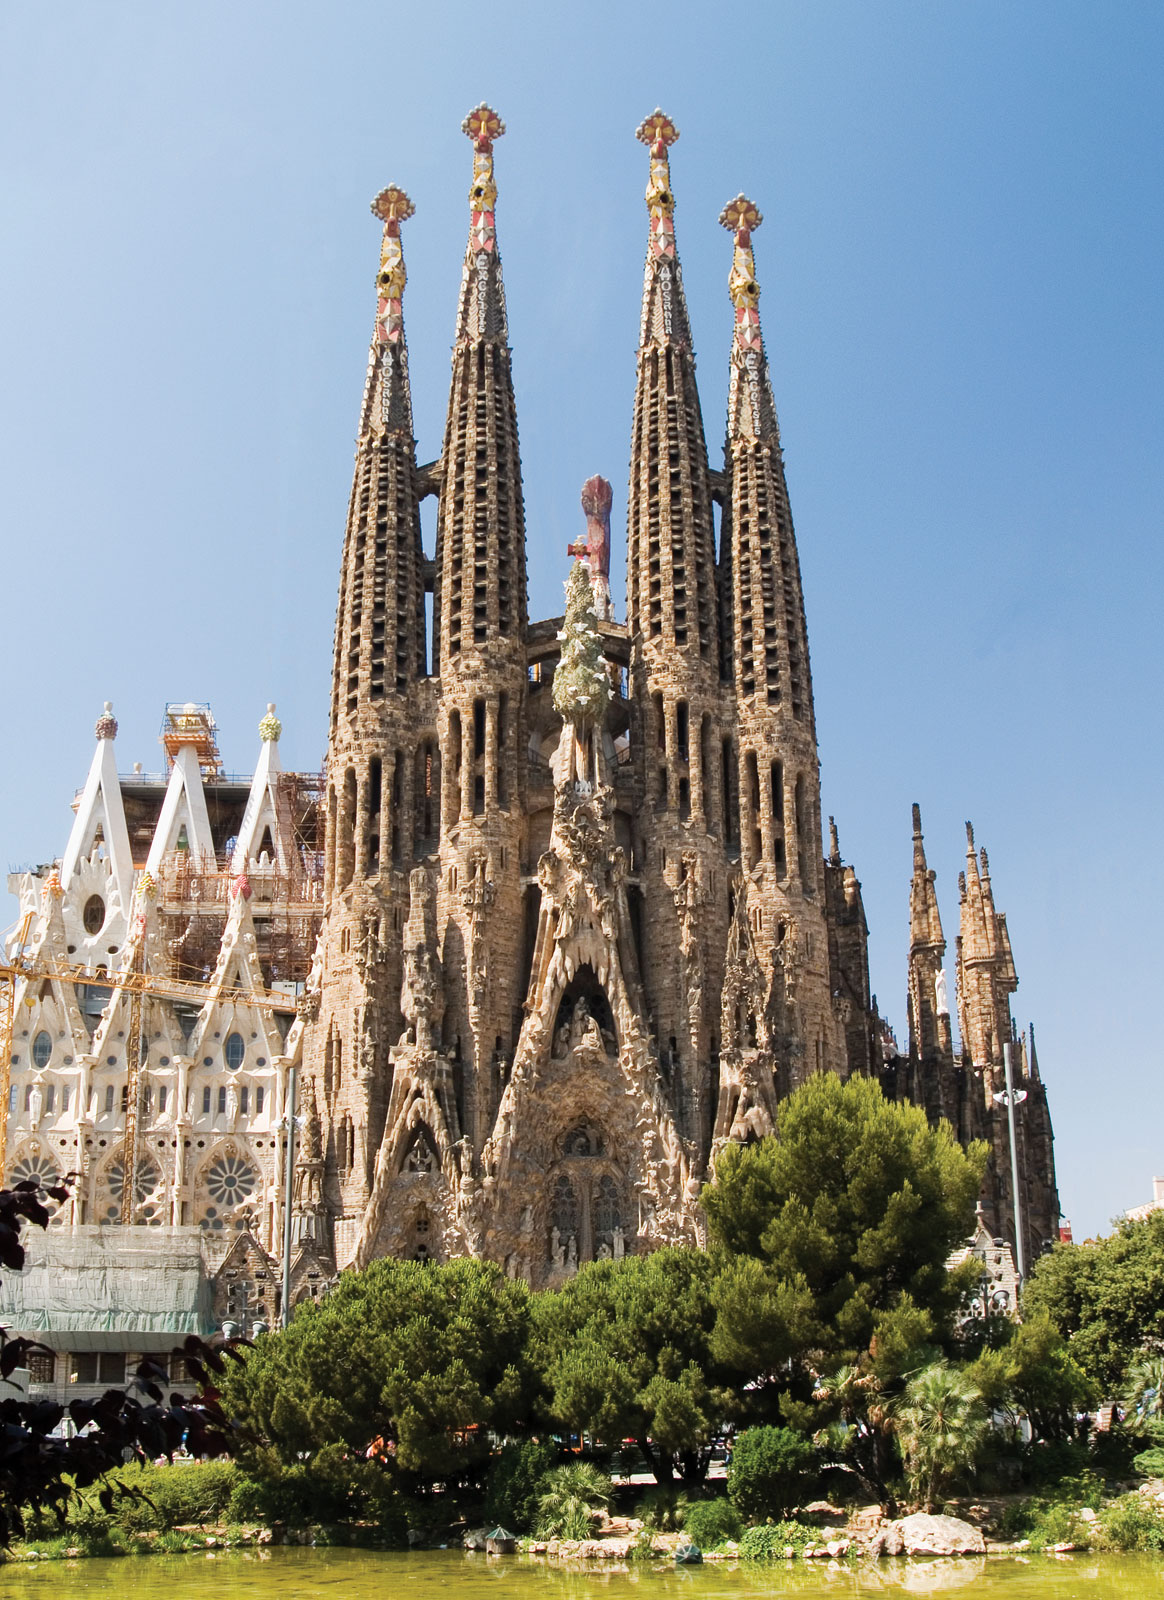
\includegraphics[height=0.9\textheight]{Figuras/Ch07/fig1.5}
\end{frame}


\begin{frame}{Introdução}
	\centering
	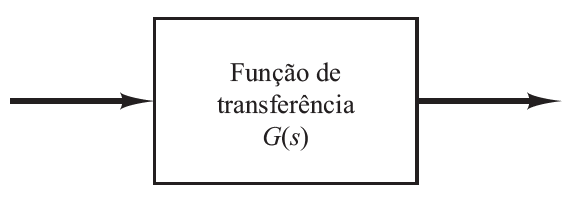
\includegraphics[width=0.95\linewidth]{Figuras/Ch07/fig1.6}
\end{frame}


\begin{frame}{Introdução}
	\begin{block}{Conceitos iniciais}
		\begin{itemize}
			\item Hoje, ao iluminarmos nossas residências, ainda temos as mesmas preocupações, como: ter uma \textbf{boa luz} para as \textbf{atividades} que fazemos em cada ambiente, os deixando \textbf{mais bonitos} e \textbf{agradáveis}, além de \textbf{destacar} detalhes da \textbf{arquitetura}, \textbf{objetos de arte} e \textbf{quadros}.
			\item Ao considerarmos \textbf{conceitos básicos de iluminação}, promovemos ambientes \textbf{belos} e mais \textbf{aconchegantes}, além de \textbf{economizarmos} em eletricidade.
		\end{itemize}
	\end{block}
\end{frame}


\begin{frame}{Introdução}
	\centering
	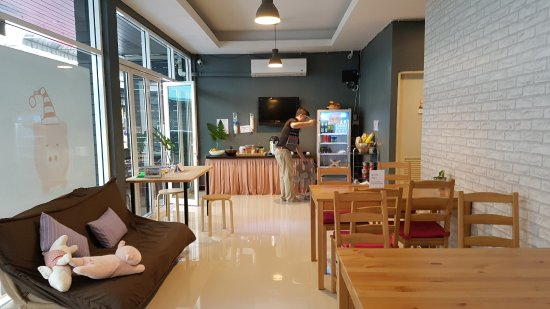
\includegraphics[width=1\linewidth]{Figuras/Ch07/fig1.7}
\end{frame}


\begin{frame}{Temperatura de Cor}
	\begin{block}{Conceitos iniciais}
		\begin{itemize}
			\item Quando falamos em luz \textbf{quente} ou \textbf{fria}, \textbf{não estamos nos referindo ao calor físico da lâmpada}, e sim a \textbf{tonalidade de cor que ela dá ao ambiente}.
			\item A \textbf{tonalidade de cor} emitida por uma fonte luminosa é denominada \textit{Temperatura de Cor} e sua unidade de medida é o \textbf{Kelvin} (\si{\kelvin}).
			\item Quanto \textbf{mais alta a temperatura de cor} de uma lâmpada, \textbf{mais clara a tonalidade de luz} emitida por ela.
			\item Ex.: uma lâmpada de temperatura de cor de \textbf{\SI{2700}{\kelvin}} tem tonalidade \textbf{suave}, uma de \textbf{\SI{6500}{\kelvin}} tem tonalidade \textbf{clara}.
			\item Em uma \textbf{residência} o \textbf{ideal} é variar entre \textbf{\num{2700} e \SI{5000}{\kelvin}} conforme o ambiente a ser iluminado.
		\end{itemize}
	\end{block}
\end{frame}


\begin{frame}{Temperatura de Cor}
	\centering
	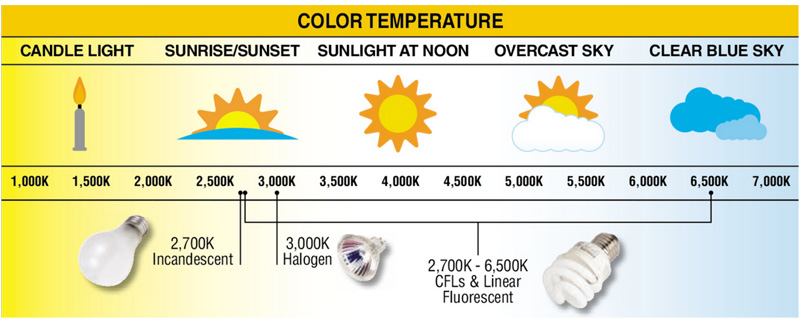
\includegraphics[width=1\linewidth]{Figuras/Ch07/fig4}
\end{frame}


\begin{frame}{Temperatura de Cor}
	\begin{block}{}
		\begin{itemize}
			\item Em uma \textbf{residência}, as \textbf{áreas sociais} e os \textbf{dormitórios} devem ter tonalidade \textbf{mais suave} ou \textbf{neutra} (\SI{3000}{\kelvin}~\SI{4000}{\kelvin}) e \textbf{salas de estudos} devem ter \textbf{tom neutro ou frio}, induzindo maior atividade.
			\item Hoje estão disponíveis no mercado lâmpadas fluorescentes com uma nova tecnologia, que permite apresentar \textbf{várias temperaturas de cor}.
			\item Antes elas só existiam em \textbf{tons claros} e estas lâmpadas \textbf{emitem menos calor}, e são erroneamente chamadas \textbf{lâmpadas frias}.
			\item Atualmente já são usadas na \textbf{casa inteira} e com \textbf{grande efeito decorativo}.
			\item As \textbf{fluorescentes compactas} estão disponíveis em temperatura de \textbf{cor clara} (\SI{6500}{\kelvin}) e também em \textbf{cor suave} (\SI{2700}{\kelvin}), semelhante às \textbf{lâmpadas incandescentes}.
		\end{itemize}
	\end{block}
\end{frame}


\begin{frame}{Temperatura de Cor}
	\centering
	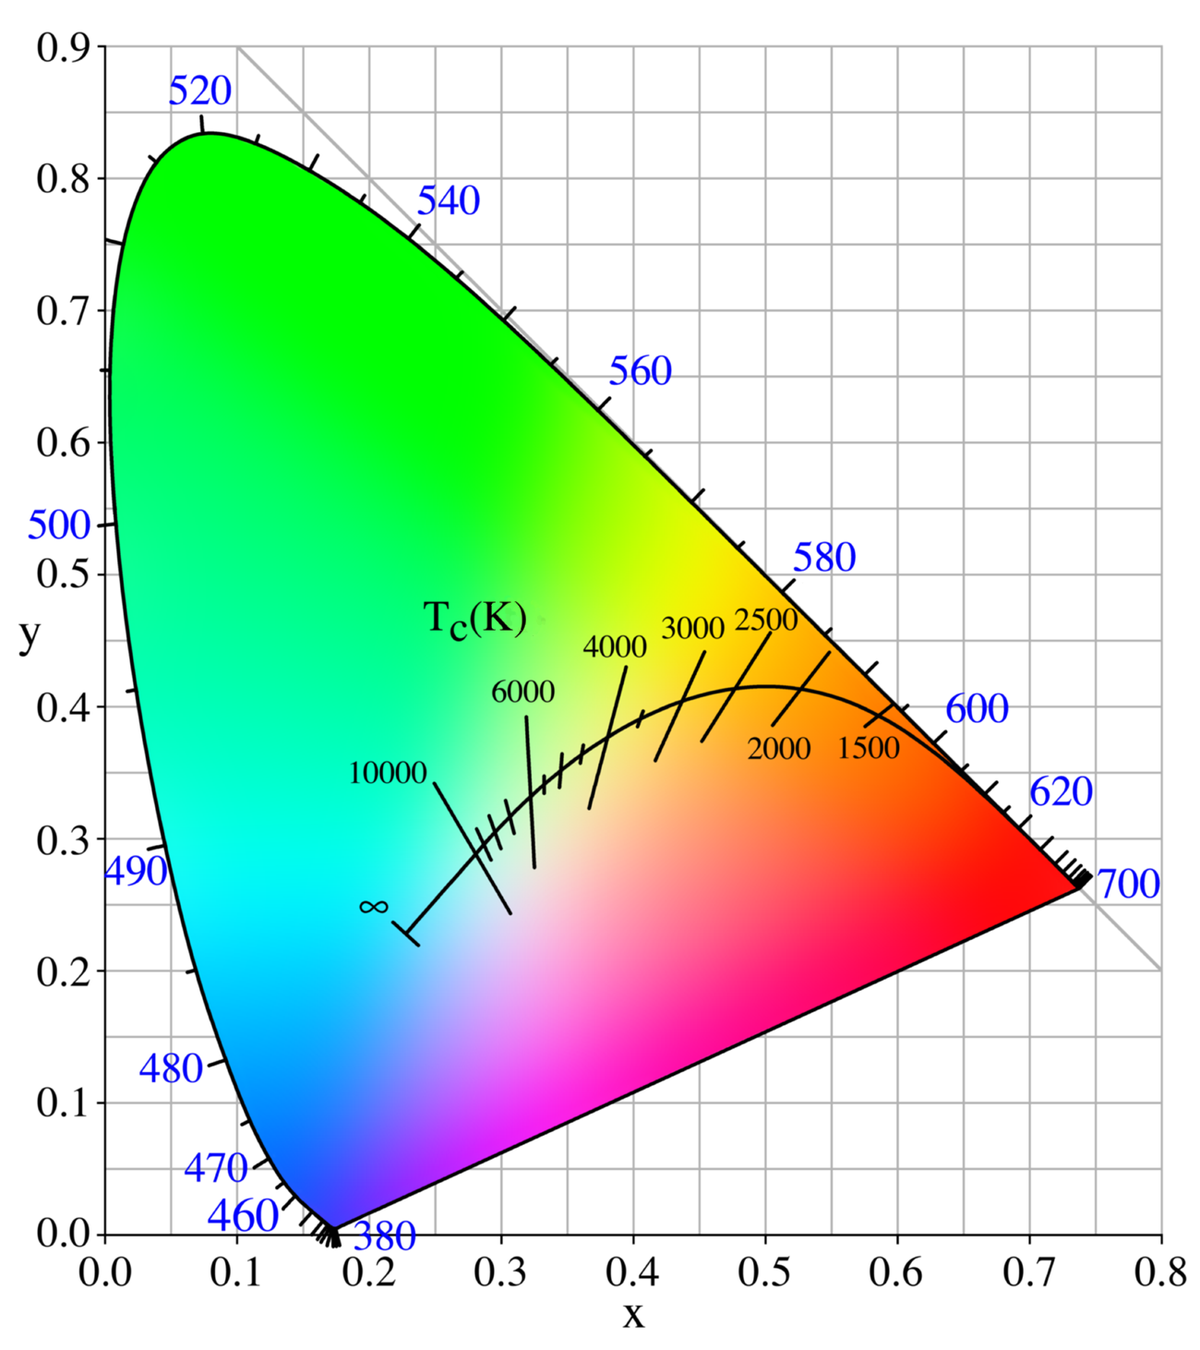
\includegraphics[height=.9\textheight]{Figuras/Ch07/fig1}
\end{frame}


\begin{frame}{Temperatura de Cor}
	\centering
	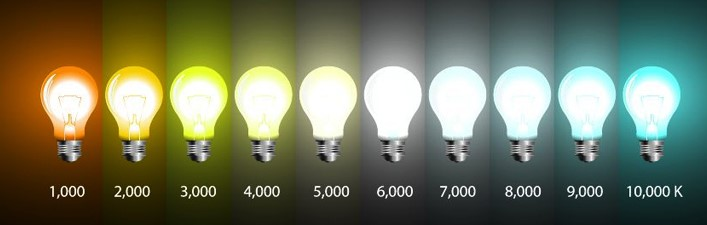
\includegraphics[width=1\linewidth]{Figuras/Ch07/fig2}
\end{frame}


\begin{frame}{Temperatura de Cor}
	\centering
	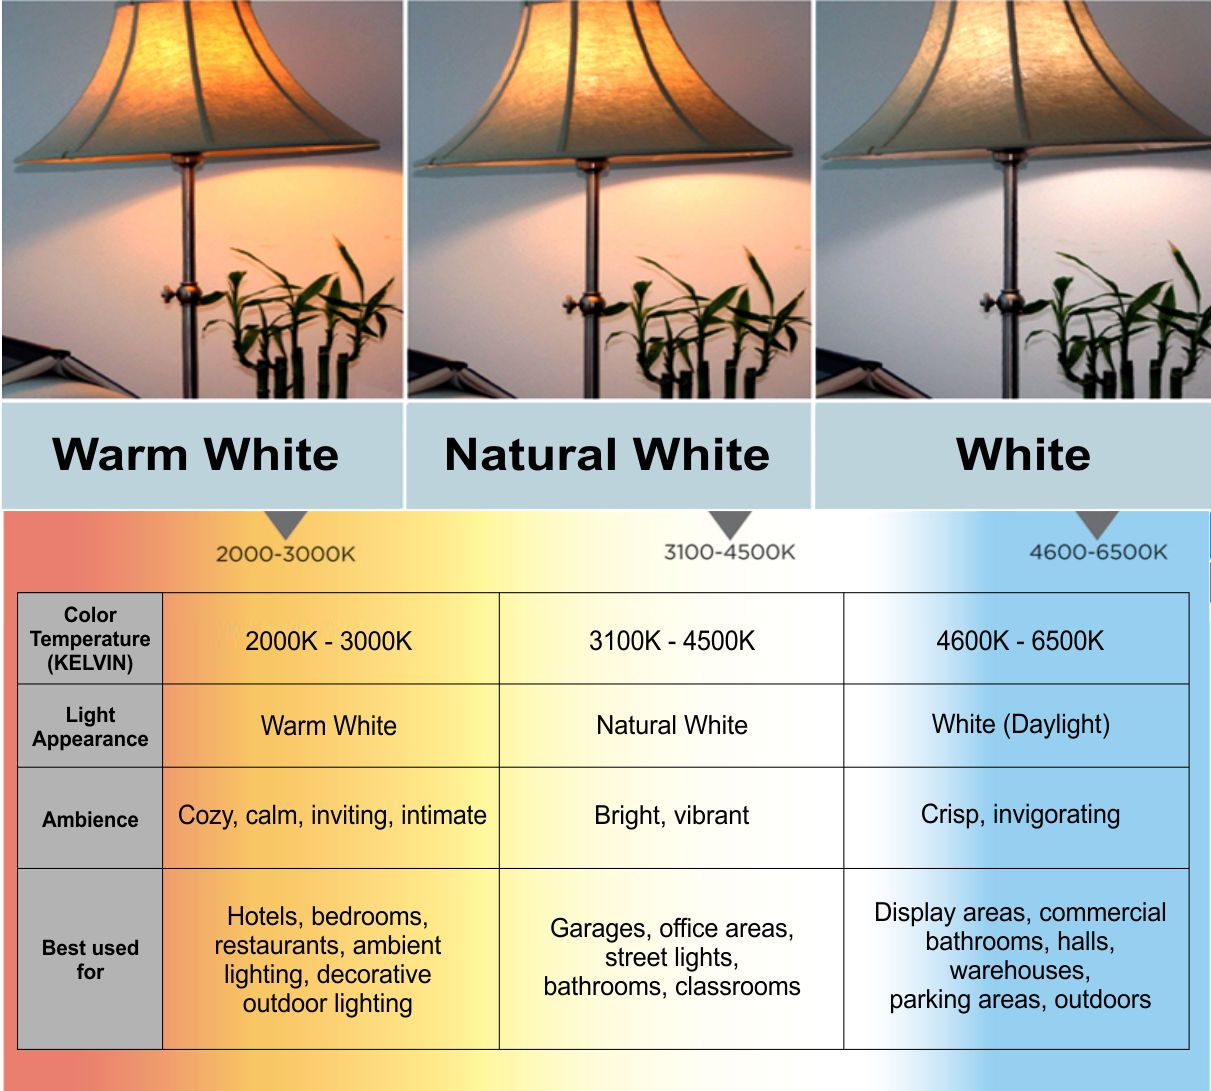
\includegraphics[width=0.7\linewidth]{Figuras/Ch07/fig3}
\end{frame}


\begin{frame}{Reprodução de Cor}
	\begin{block}{}
		\begin{itemize}
			\item Um dos pontos \textbf{mais importantes} na decoração de um ambiente é a \textbf{harmonia} e \textbf{combinação das cores}, porém isto pode ser prejudicado se não escolhermos as \textbf{lâmpadas adequadas}.
			\item A \textit{reprodução de cores} de uma lâmpada é medida por uma escala chamada \textbf{IRC} (Índice de Reprodução de Cores).
			\item Quanto \textbf{mais próximo} este índice for de \textbf{100} (equivalente à \textbf{luz solar}), \textbf{mais fielmente} as cores serão vistas na decoração.
		\end{itemize}
	\end{block}
\end{frame}


\begin{frame}{Reprodução de Cor}
	\begin{block}{}
		\begin{itemize}
			\item Isto ocorre porque, na verdade, o que enxergamos é o \textbf{reflexo da luz que ilumina os objetos}, já que no escuro não vemos as cores.
		\end{itemize}
	\end{block}

	\medskip

	\centering
	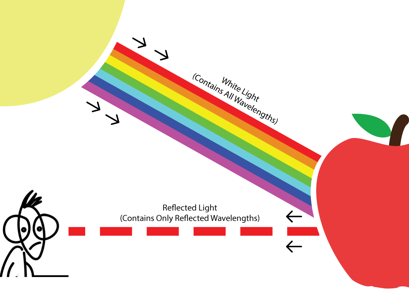
\includegraphics[width=0.7\linewidth]{Figuras/Ch07/fig5.2}

\end{frame}


\begin{frame}{Reprodução de Cor}
	\begin{block}{}
		\begin{itemize}
			\item A capacidade das lâmpadas \textbf{reproduzirem bem as cores} (IRC) \textbf{independe de sua temperatura de cor}.
			\item Existem lâmpadas com \textbf{diferentes temperaturas de cor} e que apresentam o \textbf{mesmo IRC}.
			\item Em áreas \textbf{residenciais} e \textbf{comerciais} devemos utilizar lâmpadas com \textbf{boa reprodução de cores} (IRC acima de 80), pois a cor é \textbf{fundamental} para o \textbf{conforto e beleza do ambiente}.
		\end{itemize}
	\end{block}
\end{frame}


\begin{frame}{Reprodução de Cor}
	\centering
	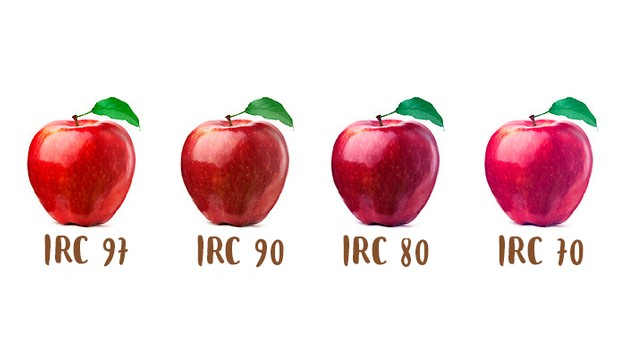
\includegraphics[width=1\linewidth]{Figuras/Ch07/fig6}
\end{frame}


\begin{frame}{Reprodução de Cor}
	\centering
	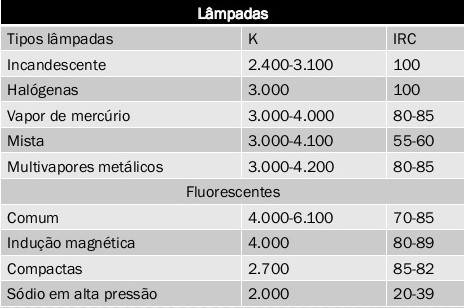
\includegraphics[width=0.9\linewidth]{Figuras/Ch07/fig7}
\end{frame}


\begin{frame}{Reprodução de Cor}
	\centering
	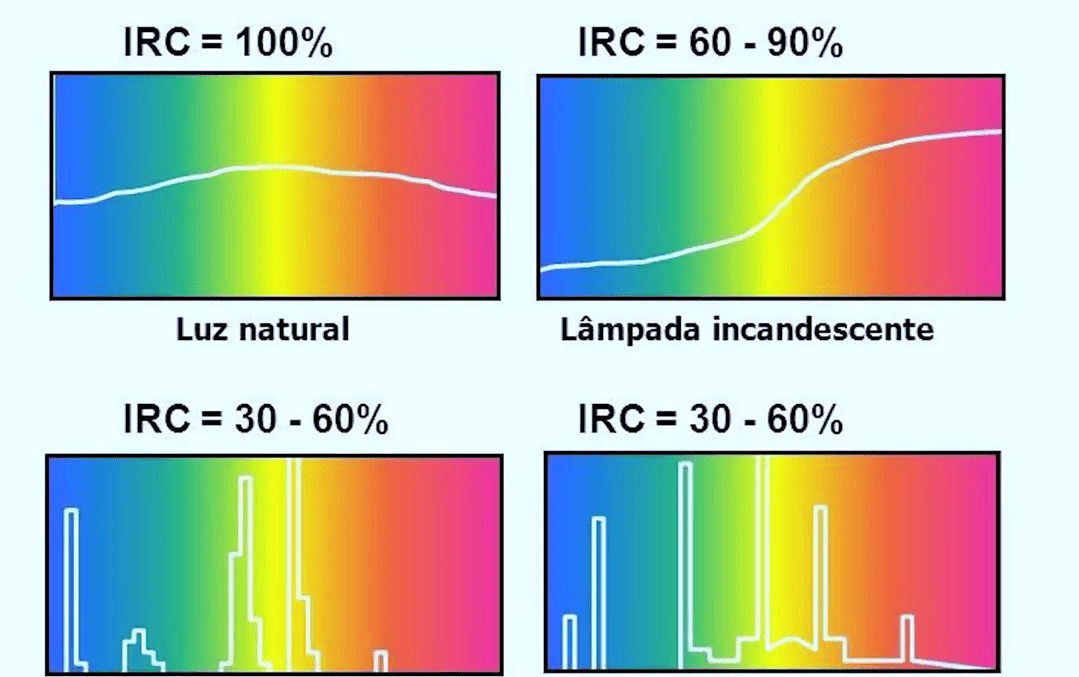
\includegraphics[width=0.9\linewidth]{Figuras/Ch07/fig5.1}
\end{frame}


\begin{frame}{Eficiência e Economia}
	\begin{block}{}
		\begin{itemize}
			\item Provavelmente estas não são as primeiras palavras que vêm a sua mente quando você pensa em comprar lâmpadas para iluminar sua casa.
			\item Geralmente você está pensando em \textbf{beleza} e \textbf{destaque} para sua decoração ou ainda em deixar a casa \textbf{clara} e \textbf{bem iluminada}.
			\item A \textit{eficiência} de uma lâmpada é a maneira como ela \textbf{consome energia elétrica}.
			\item Nas lâmpadas \textbf{incandescentes} e \textbf{halógenas}, \textbf{80\%} da energia utilizada é transformada em \textbf{calor} e \textbf{apenas 15\% gera luz}.
			\item Toda esta energia transformada em calor é \textbf{lançada no ambiente}, causando \textbf{aumento da temperatura} e \textbf{desconforto}.
			\item As lâmpadas \textbf{fluorescentes} e as \textbf{fluorescentes compactas} (\textit{Energy Saver} - economizadoras de energia) tem \textbf{outra maneira de funcionar}, produzindo \textbf{mais luz} e \textbf{emitindo pouco calor}.
		\end{itemize}
	\end{block}
\end{frame}


\begin{frame}{Eficiência e Economia}
	\begin{block}{}
		\begin{itemize}
			\item Então, podemos dizer que uma lâmpada \textbf{é mais eficiente} à medida que a \textbf{maior parte da energia consumida por ela é destinada à produção de luz}.
			\item Estima-se que a iluminação seja responsável por uma \textbf{pequena parcela do consumo de energia} do lar (\textbf{entre 10\% e 20\%}).
			\item Porém esta parcela pode ser \textbf{ainda mais reduzida} com a \textbf{troca das lâmpadas convencionais por lâmpadas de alta tecnologia} como as Energy Saver.
			\item Isso \textbf{sem nenhum prejuízo no nível de iluminação} e com uma \textbf{série de benefícios}, como por exemplo: a \textbf{redução do volume de calor lançado no ambiente} e a \textbf{diminuição da troca de lâmpadas}, pois elas \textbf{além da economia no consumo}, \textbf{têm a vida útil maior que as lâmpadas incandescentes}.
		\end{itemize}
	\end{block}
\end{frame}


\begin{frame}{Eficiência e Economia}
	\centering
	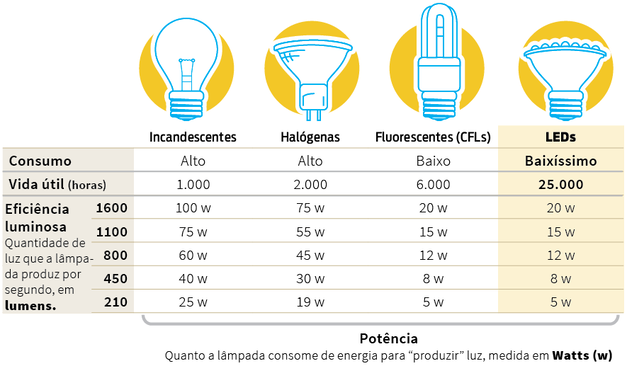
\includegraphics[width=0.9\linewidth]{Figuras/Ch07/fig8}
\end{frame}


\begin{frame}{Eficiência e Economia}
	\begin{block}{Lâmpada incandescente}
		\begin{itemize}
			\item Essas lâmpadas funcionam pelo princípio de \textbf{aquecimento de um filamento elétrico} (similar à \textbf{resistência} de um chuveiro), que devido à sua composição \textbf{emite luz a uma dada temperatura} (efeito Joule).
		\end{itemize}
	\end{block}

	\bigskip

	\centering
	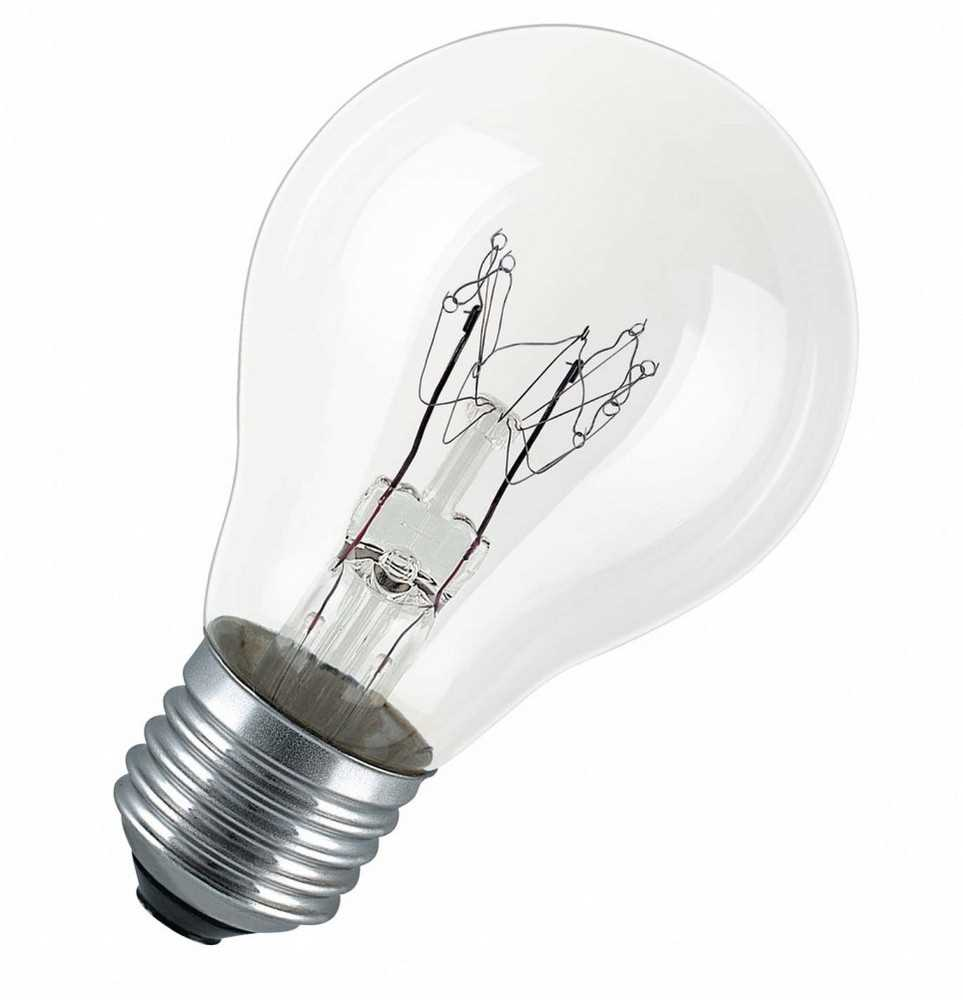
\includegraphics[height=0.5\textheight]{Figuras/Ch07/fig9}
\end{frame}


\begin{frame}{Eficiência e Economia}
	\begin{block}{Lâmpada incandescente}
		\begin{itemize}
			\item São os modelos mais \textbf{antigos} e \textbf{comuns}, tem como vantagem o \textbf{baixo custo} e a emissão de \textbf{muita luz}, porém possuem \textbf{alto consumo de energia}, visto que boa parte da energia que chega até ela é convertida em \textbf{calor}.
			\item Talvez por esse motivo sua \textbf{vida útil} também é \textbf{baixa}.
			\item Este tipo de lâmpada deverá \textbf{desaparecer} nos próximos anos.
		\end{itemize}
	\end{block}

	%	\bigskip

	\centering
	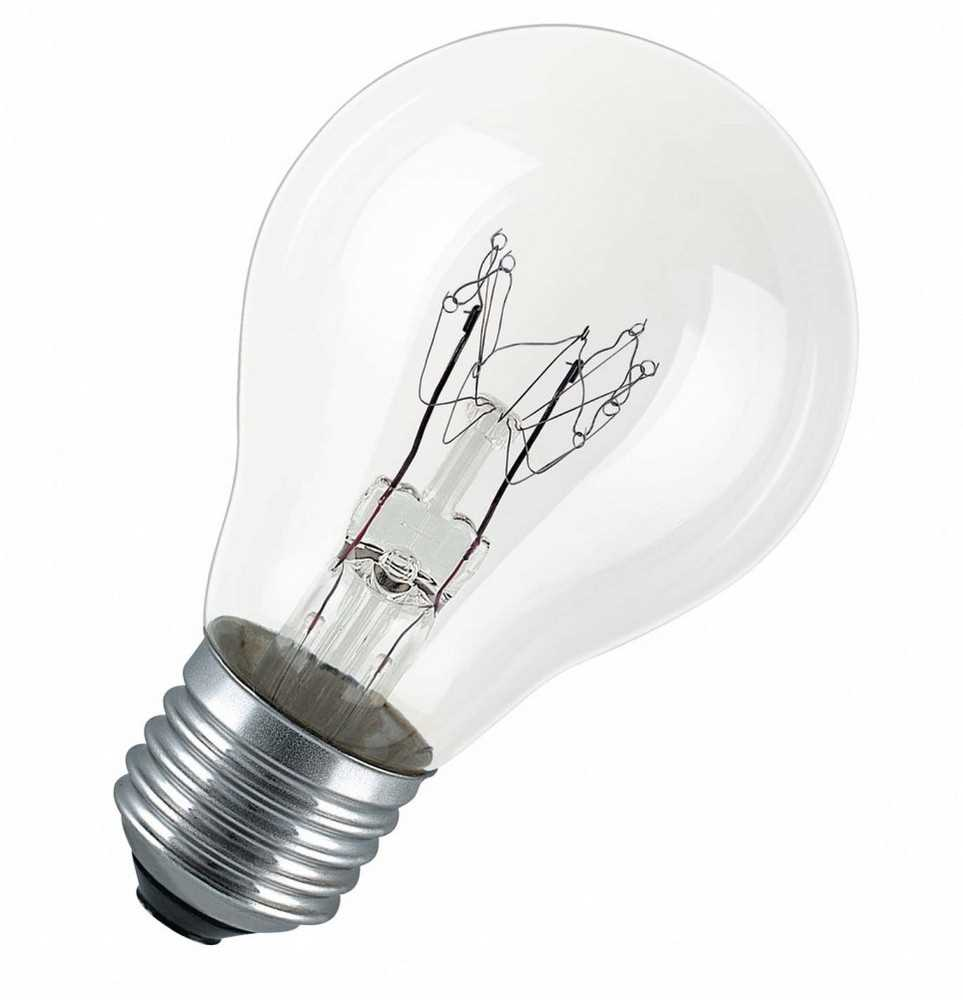
\includegraphics[height=0.45\textheight]{Figuras/Ch07/fig9}
\end{frame}


\begin{frame}{Eficiência e Economia}
	\begin{block}{Lâmpada fluorescente}
		\begin{itemize}
			\item A lâmpada fluorescente funciona através do \textbf{distúrbio de gases inertes} que, quando sofrem \textbf{descargas eletrônicas}, emitem \textbf{luz}.
			\item O modelo fluorescente foi criado por Nikola Tesla em 1938.
			\item Ela possui \textbf{melhor eficiência energética} por emitir mais energia em forma de \textbf{luz} do que \textbf{calor}.
		\end{itemize}
	\end{block}

	\centering
	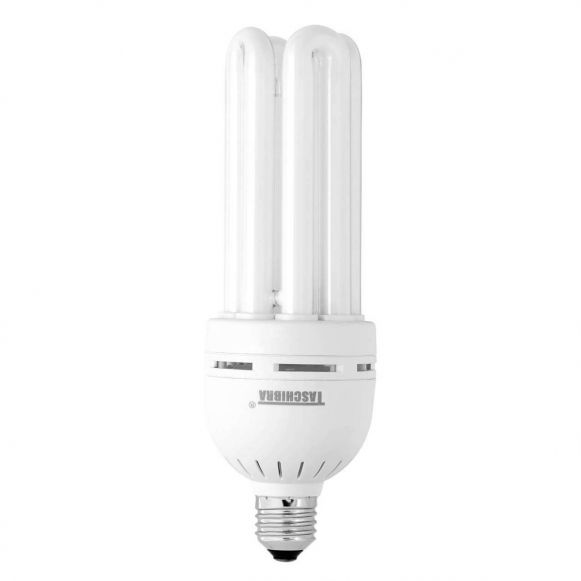
\includegraphics[height=0.5\textheight]{Figuras/Ch07/fig10}
\end{frame}


\begin{frame}{Eficiência e Economia}
	\begin{block}{Lâmpada fluorescente}
		\begin{itemize}
			\item A lâmpada fluorescente tornou-se o \textbf{padrão} para muitas pessoas, pois ela \textbf{consome menos energia} que a incandescente, mas ainda assim \textbf{tem um consumo considerável}.
			\item Ela emite uma \textbf{luz branca e forte} e pode ser usada em \textbf{todos os ambientes}.
			\item Um detalhe importante é que este tipo de lâmpada usa \textbf{mercúrio e fósforo} portanto \textbf{não pode ser descartada de qualquer maneira}, pois \textbf{provoca danos ao meio ambiente}.
		\end{itemize}
	\end{block}

	\centering
	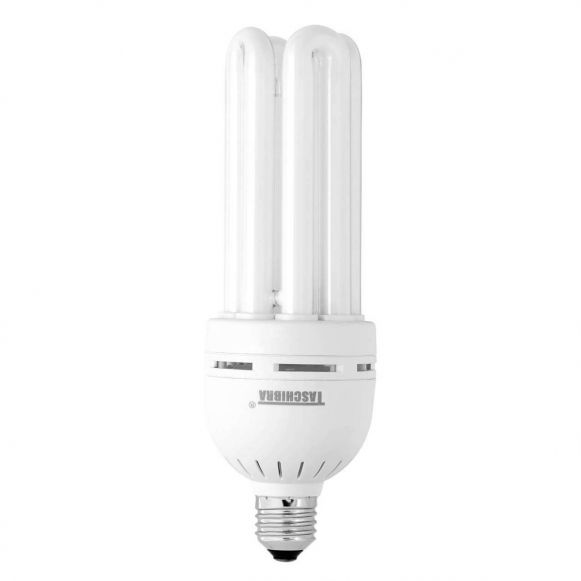
\includegraphics[height=0.35\textheight]{Figuras/Ch07/fig10}
\end{frame}


\begin{frame}{Eficiência e Economia}
	\begin{block}{Lâmpada de LED}
		\begin{itemize}
			\item A lâmpada de LED é um \textbf{diodo}, que é uma junção de \textbf{cristais dopados} (alterados), de tal forma que, quando percorridos por corrente elétrica em um sentido específico \textbf{podem emitir luz}.
		\end{itemize}
	\end{block}

	\bigskip

	\centering
	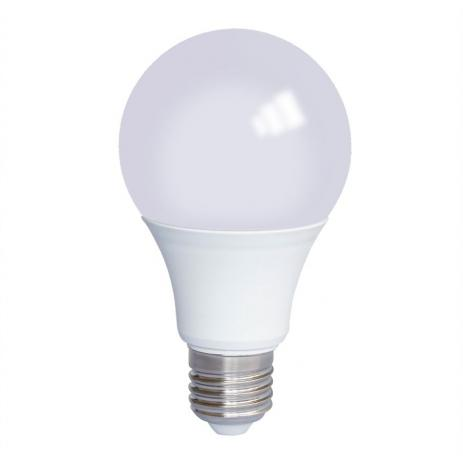
\includegraphics[height=0.5\textheight]{Figuras/Ch07/fig11}
\end{frame}


\begin{frame}{Eficiência e Economia}
	\begin{block}{Lâmpada de LED}
		\begin{itemize}
			\item As lâmpadas de LED são as \textbf{mais modernas}.
			\item Sua tecnologia moderna permite um \textbf{baixíssimo consumo de energia} que a tornam muito atraente.
			\item Como desvantagens temos ainda o seu \textbf{altíssimo custo} e a \textbf{baixa luminosidade}, a menos que seja usada a \textbf{super LED}.
		\end{itemize}
	\end{block}

	\centering
	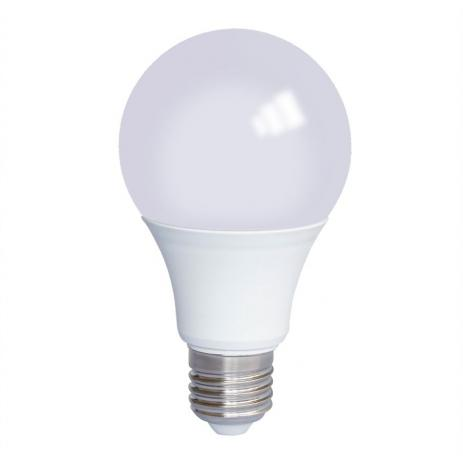
\includegraphics[height=0.5\textheight]{Figuras/Ch07/fig11}
\end{frame}


\section*{Exercícios}
\frame{
	\frametitle{Exercícios}
	\begin{block}{}
		01. Elabore um esquema de iluminação para sua casa.

		\bigskip

		02. Responda quais as recomendações gerais de lâmpada cada caso:

		\medskip

		(a) Quarto

		\medskip

		(b) Escritório

		\medskip

		(c) Sala de estar

		\medskip

		(d) Salão de festas
	\end{block}
}

\section*{Referências}

\frame{
	\frametitle{Referências e Exercícios Complementares}
	\begin{itemize}
		\item CREDER, Hélio; Instalações Elétricas, 14ª edição, Editora LTC, Rio de Janeiro, 2004.
		\item Manual de Instalações Elétricas - Prysmian.
	\end{itemize}
	%\centering{\alert{Página 36 - \textbf{1.6.1 até 1.6.5, 1.6.17 até 1.6.19}}} \\
	%	\centering{\alert{Lista de exercícios 01}}
}